%%%%%%%%%%%%%%%%%%%%%%%%%%%%%%%%%%%%%%%%%%%%%%%%%%%%%%%%%%%%%%%%%%%%%%%%%%%%%%%%
%2345678901234567890123456789012345678901234567890123456789012345678901234567890
%        1         2         3         4         5         6         7         8

\documentclass[letterpaper, 10 pt, conference]{ieeeconf}  % Comment this line out if you need a4paper

%\documentclass[a4paper, 10pt, conference]{ieeeconf}      % Use this line for a4 paper

\IEEEoverridecommandlockouts                              % This command is only needed if 
                                                          % you want to use the \thanks command

\overrideIEEEmargins                                      % Needed to meet printer requirements.

%In case you encounter the following error:
%Error 1010 The PDF file may be corrupt (unable to open PDF file) OR
%Error 1000 An error occurred while parsing a contents stream. Unable to analyze the PDF file.
%This is a known problem with pdfLaTeX conversion filter. The file cannot be opened with acrobat reader
%Please use one of the alternatives below to circumvent this error by uncommenting one or the other
%\pdfobjcompresslevel=0
%\pdfminorversion=4

% See the \addtolength command later in the file to balance the column lengths
% on the last page of the document

% The following packages can be found on http:\\www.ctan.org
\usepackage{graphics} % for pdf, bitmapped graphics files
\usepackage{epsfig} % for postscript graphics files
\usepackage{mathptmx} % assumes new font selection scheme installed
\usepackage{times} % assumes new font selection scheme installed
\usepackage{amsmath} % assumes amsmath package installed
\usepackage{amssymb}  % assumes amsmath package installed

\title{\LARGE \bf
ROB 530 Project Proposal: \\ Terrain-Aided Proprioceptive Localization for Snake Robots
}

\author{Riley Bridges, Quintin Dwight, Christian Foreman, and Andrew Scheffer% <-this % stops a space
% \thanks{*This work was not supported by any organization}% <-this % stops a space
% \thanks{$^{1}$Albert Author is with Faculty of Electrical Engineering, Mathematics and Computer Science,
%         University of Twente, 7500 AE Enschede, The Netherlands
%         {\tt\small albert.author@papercept.net}}%
% \thanks{$^{2}$Bernard D. Researcheris with the Department of Electrical Engineering, Wright State University,
%         Dayton, OH 45435, USA
%         {\tt\small b.d.researcher@ieee.org}}%
}

\begin{document}

\maketitle
\thispagestyle{empty}
\pagestyle{empty}

%%%%%%%%%%%%%%%%%%%%%%%%%%%%%%%%%%%%%%%%%%%%%%%%%%%%%%%%%%%%%%%%%%%%%%%%%%%%%%%%
% \begin{abstract}

% TODO

% \end{abstract}

%%%%%%%%%%%%%%%%%%%%%%%%%%%%%%%%%%%%%%%%%%%%%%%%%%%%%%%%%%%%%%%%%%%%%%%%%%%%%%%%
\section{Project Objectives}
We aim to develop a state estimation and localization algorithm for a mobile snake robot (shown in Figure \ref{fig:snake_robot}) operating in an environment with known terrain. Specifically, our objective is to estimate the robot's 3D pose and the configuration of its joints. This algorithm will be tested and evaluated in simulation, using a 3D model and physics engine to replicate the robot's real world behavior. The robot will be equipped with a six DoF IMU (three axis accelerometer and three axis gyroscope) and a contact/force sensor attached to each link, as well as an absolute rotary encoder attached to each joint. A terrain map will be used to provide information about the environment. Several different state estimation algorithms will be implemented, and each one will be evaluated based on its accuracy and robustness to sensor noise and drift.

\begin{figure}[h]
    \centering
    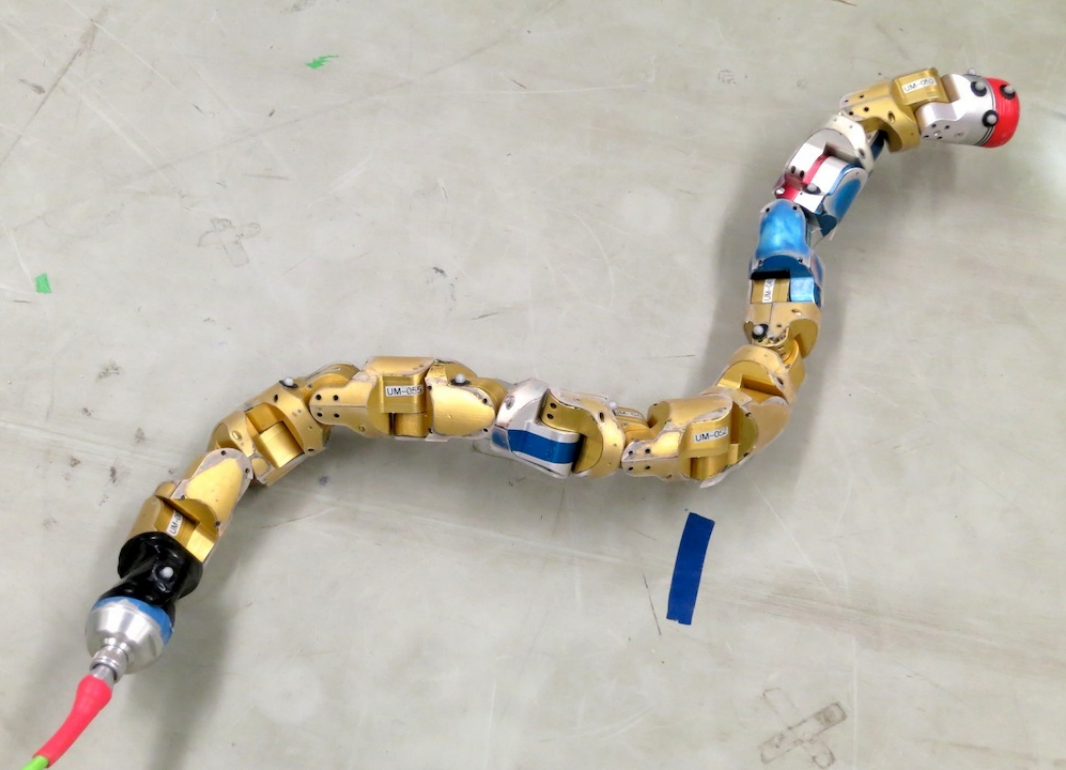
\includegraphics[width=0.7\linewidth]{snake_robot.png}
    \caption{Example of a snake robot \cite{c1}.}
    \label{fig:snake_robot}
\end{figure}

\section{Technical Approach}

The snake robot's orientation and joint configuration will be estimated separately from its position. An EKF will be used to estimate orientation and joint configuration, with a formulation similar to those in \cite{c1} and \cite{c2}. In addition to orientation and joint angles, serpentine gait parameters will be included in the state vector in order to simplify modeling of the robot's kinematics. Angular velocity commands for each joint will be used in the prediction step, while IMU and encoder measurements will be used in the correction step. 

Instead of attaching the body frame to a single link of the snake robot, a virtual body frame is defined at the center of mass and aligned to the principal moments of inertia of the snake. This helps to separate the configuration of individual joints from the overall orientation of the robot.

A particle filter will be used to estimate the 3D position of the robot relative to an inertial map frame. Estimated gait parameters from the EKF will be used to propagate each particle forward, and predicted contact forces will be compared to the measured forces in order to weight the particles in the correction step.  
These predicted contact forces will be computed by projecting a model of the snake robot into the terrain map, using the particles' position estimates and the orientation estimate from the EKF.

\section{Novelty}
While this project is built off of the work from \cite{c1} and \cite{c2}, we will provide the following novel contributions:
\begin{itemize}
    \item Estimation of the full 3D pose of the snake rather than just the 3D orientation.
    \item Use of a terrain map to provide correction information for snake positioning.
    \item Use and evaluation of particle filtering for snake robot state estimation.
\end{itemize} 

\section{Milestones and Work Distribution}
Table \ref{tab:milestones} lays out our projected timeline. While everyone plans to take part in most implementation steps, each major component will have a team member in charge.
\begin{table}[h]
    \centering
    \caption{Target timeline for project}
    \begin{tabular}{|c|c|c|} \hline 
         \textbf{Date}&  \textbf{Key Milestones} & \textbf{Person}\\ \hline 
         March 15th&PyBullet simulation with snake robot model& Quintin\\\hline
         March 29th& Orientation and joint configuration EKF & Riley \\ \hline
         April 12th&Particle filter framework and prediction step & Drew \\ \hline
         April 12th& Particle filter correction step & Christian \\ \hline
         April 12th& Begin data analysis and final reports & All \\ \hline
        April 19th&Video submission & All \\ \hline
        April 19th&Paper submission & All \\ \hline
    \end{tabular}
    \label{tab:milestones}
\end{table}

\section{Expected Outcomes}
Once our work is complete, we aim to have the following deliverables:
\begin{enumerate}
    \item Simulator that can load a terrain map and simulate the physics of a snake robot moving within it.
    \item Implementation of an algorithm to estimate the 3D pose of the snake.
    \item Analysis of our algorithm's performance vs. simulator ground truth.
\end{enumerate}

\begin{thebibliography}{99}
    \bibitem{c1} Rollinson, D, Choset, H, \& Tully, S. "Robust State Estimation With Redundant Proprioceptive Sensors." Proceedings of the ASME 2013 Dynamic Systems and Control Conference. Volume 3: Nonlinear Estimation and Control; Optimization and Optimal Control; Piezoelectric Actuation and Nanoscale Control; Robotics and Manipulators; Sensing; System Identification (Estimation for Automotive Applications, Modeling, Therapeutic Control in Bio-Systems); Variable Structure/Sliding-Mode Control; Vehicles and Human Robotics; Vehicle Dynamics and Control; Vehicle Path Planning and Collision Avoidance; Vibrational and Mechanical Systems; Wind Energy Systems and Control. Palo Alto, California, USA. October 21–23, 2013. V003T40A005. ASME. https://doi.org/10.1115/DSCC2013-3873

    \bibitem{c2} D. Rollinson, A. Buchan and H. Choset, "State estimation for snake robots," 2011 IEEE/RSJ International Conference on Intelligent Robots and Systems, San Francisco, CA, USA, 2011, pp. 1075-1080, doi: 10.1109/IROS.2011.6095052.
\end{thebibliography}

\end{document}
